\section{Sri Rahayu(1174015)}
\subsection{PYSHP Reader}
\begin{enumerate}
    \item Buatlah Script Python dan jelaskan berbaris
    \lstinputlisting[firstline=8, lastline=11]{src/1174015/3/1174015.py}
    \hfill\break
    \begin{figure}[H]
		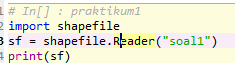
\includegraphics[width=4cm]{figures/1174015/3/No1.png}
		\centering
		\caption{Hasil SHP Reader Soal 1}
    \end{figure}
    
    \item Buatlah Script Python dan jelaskan berbaris
    \lstinputlisting[firstline=13, lastline=15]{src/1174015/3/1174015.py}
    \hfill\break
    \begin{figure}[H]
		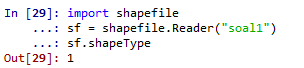
\includegraphics[width=4cm]{figures/1174015/3/No2.png}
		\centering
		\caption{Hasil SHP Reader Soal 2}
    \end{figure}
    
    \item Buatlah Script Python dan jelaskan berbaris
    \lstinputlisting[firstline=17, lastline=19]{src/1174015/3/1174015.py}
    \hfill\break
    \begin{figure}[H]
		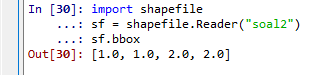
\includegraphics[width=4cm]{figures/1174015/3/No3.png}
		\centering
		\caption{Hasil SHP Reader Soal 3}
    \end{figure}
    
    \item Buatlah Script Python dan jelaskan berbaris
    \lstinputlisting[firstline=21, lastline=24]{src/1174015/3/1174015.py}
    \hfill\break
    \begin{figure}[H]
		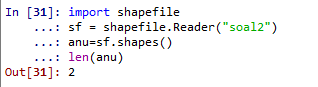
\includegraphics[width=4cm]{figures/1174015/3/No4.png}
		\centering
		\caption{Hasil SHP Reader Soal 4}
    \end{figure}
    
    \item Buatlah Script Python dan jelaskan berbaris
    \lstinputlisting[firstline=18, lastline=22]{src/1174015/3/1174015.py}
    \hfill\break
    \begin{figure}[H]
		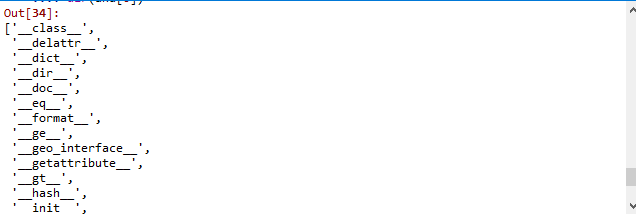
\includegraphics[width=4cm]{figures/1174015/3/No5.png}
		\centering
		\caption{Hasil SHP Reader Soal 5 Codingan}
    \end{figure}
    
    \item Buatlah Script Python dan jelaskan berbaris
    \lstinputlisting[firstline=32, lastline=35]{src/1174015/3/1174015.py}
    \hfill\break
    \begin{figure}[H]
		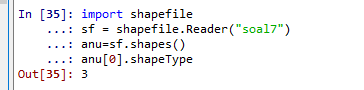
\includegraphics[width=4cm]{figures/1174015/3/No6.png}
		\centering
		\caption{Hasil SHP Reader Soal 6}
    \end{figure}

    \item Buatlah Script Python dan jelaskan berbaris
    \lstinputlisting[firstline=37, lastline=41]{src/1174015/3/1174015.py}
    \hfill\break
    \begin{figure}[H]
		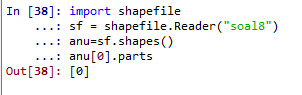
\includegraphics[width=4cm]{figures/1174015/3/No7.png}
		\centering
		\caption{Hasil SHP Reader Soal 7}
    \end{figure}

    \item Buatlah Script Python dan jelaskan berbaris
    \lstinputlisting[firstline=43, lastline=46]{src/1174015/3/1174015.py}
    \hfill\break
    \begin{figure}[H]
		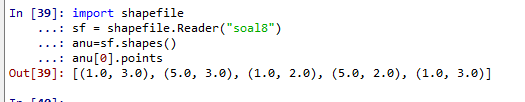
\includegraphics[width=4cm]{figures/1174015/3/No8.png}
		\centering
		\caption{Hasil SHP Reader Soal 8}
    \end{figure}

    \item Buatlah Script Python dan jelaskan berbaris
    \lstinputlisting[firstline=48, lastline=51]{src/1174015/3/1174015.py}
    \hfill\break
    \begin{figure}[H]
		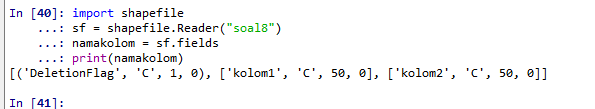
\includegraphics[width=4cm]{figures/1174015/3/No9.png}
		\centering
		\caption{Hasil SHP Reader Soal 9}
    \end{figure}

    \item Buatlah Script Python dan jelaskan berbaris
    \lstinputlisting[firstline=53, lastline=56]{src/1174015/3/1174015.py}
    \hfill\break
    \begin{figure}[H]
		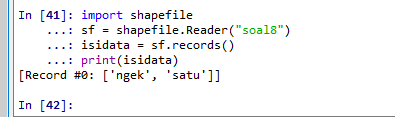
\includegraphics[width=4cm]{figures/1174015/3/No10.png}
		\centering
		\caption{Hasil SHP Reader Soal 10}
    \end{figure}

    \item Buatlah Script Python dan jelaskan berbaris
    \item \lstinputlisting[firstline=58, lastline=62]{src/1174015/3/1174015.py}
    \hfill\break
    \begin{figure}[H]
		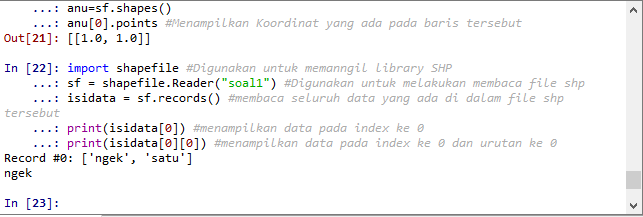
\includegraphics[width=4cm]{figures/1174015/3/No11.png}
		\centering
		\caption{Hasil SHP Reader Soal 11}
    \end{figure}
\end{enumerate}
\subsection{Link Youtube}
\href{ttps://https://youtu.be/56zCUS48CWU}{Video Youtube}